%!TEX root = ../research_proposal.tex

\section{BIANCA - Bug Insertion ANticipation by Clone Analysis at commit time\label{sec:BIANCA}}

{\tt BIANCA} (Bug Insertion ANticipation by Clone Analysis at commit time) is the final piece of the proposed ecosystem and, as such, the final failsafe that prevent developer to ship code that we know to be sub-optimum or to be at the very root of issues.

\subsection{Motivation\label{sec:bianca-motivation}}

Many tools exist to prevent a developer to ship {\it bad} code \cite{Dangel2000,Hovemeyer2007,Moha2010} or to identify {\it bad} code after executions (e.g in test or production environment) \cite{Nayrolles,Nayrolles2013a}.
However, these tools rely on metrics and rules to statically and/or dynamically identify sub-optimum code.

\subsection{The {\tt BIANCA} approach\label{sec:bianca-approach}}

{\tt BIANCA} is different than the tool presented in \ref{sec:bianca-motivation} because, as {\tt RESEMBLE} it fetch its data into the common knowledge of hundreds of thousands of projects and developers.
More specifically, {\tt BIANCA} mine and analyze the change pattern in commits and match it against past commit known to have introduce a defect in the code (or that have just been replaced by better implementation). Figure \ref{fig:bianca-approach} present an overview of our approach.

\begin{figure}[h!]
  \centering
    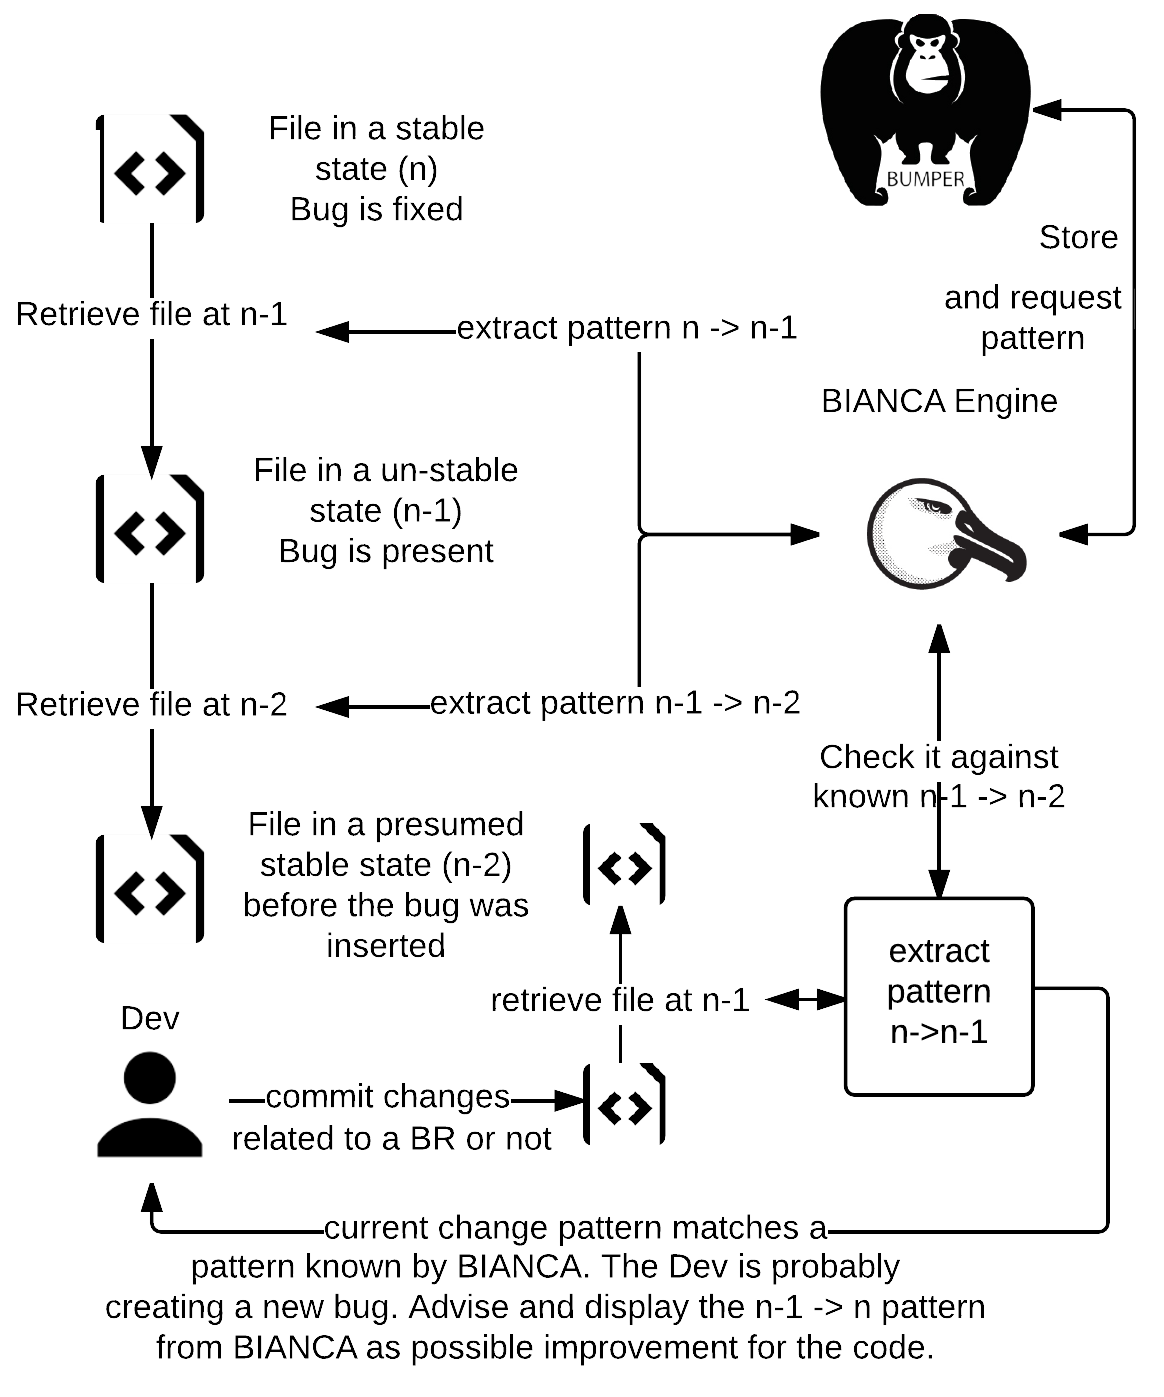
\includegraphics{media/bianca-approach.png}
    \caption{The BIANCA Approach
    \label{fig:bianca-approach}}
\end{figure}

{\tt BIANCA} builds a model where each issue stored in {\tt BUMPER} three versions of the same file.
The first version $n$ is called the {\it stable state} because the code of this version was used to fix an issue.
The $n-1$ version, however, is called the {\it unstable state} as it was marked as containing an issue.
Finally, the third state is called the {\it before state} and represent the file before the introduction of the bug.
Hereafter, we refer at the {\it before state} with the $n-2$ name.
{\tt BIANCA} extracts the change pattern form $n-2$ to $n-1$ and from $n-1$ to $n$ and generate the changes to go directly from $n-2$ to $n$.

When a developer commits new modifications, {\tt BIANCA} extracts the change pattern from the version $n_{dev}$ (current version) and $n-1_{dev}$ (version before modification) of the developer's source code and compare this change pattern to known $n-2$ to $n-1$ patterns.
If $n_{dev}$ to $n-1_{dev}$ matches a $n-2$ to $n-1$ then it means that the developer is inserting a known defect in the source code.
In such a case, {\tt BIANCA} will propose the related $n-1$ to $n$ pattern to the developer, so s/he could improve the source code and will show the related $n-2$ for the $n$ pattern so the developer will learn how to s/he should have modified the code in the first place. Moreover, if the issue was previously reproduced by {\tt JCHARMING}, then {\tt BIANCA} will display the step to reproduce it.

To extract the change patterns and compare them, we used the same technique as the one presented in sections \ref{sec:resemble-normalization} and \ref{sec:resemble-comparing} with new normalizations.
The third and the fourth normalizations are removing all {\it less} important calls in the normalization one and two of {\tt RESEMBLE}.
We classify a call as less-important if, for example, it only does display-related functionalities such as generating HTML or printing something to the console. Finally, the fourth normalization will transform the code to an intermediate language of our own that will allow us to compare source code implemented in different programming languages.

Then, as in {\tt RESEMBLE}, if the LCS is above a user-defined threshold, then a warning is raised by {\tt BIANCA} alerting the developer that the commit is suspected to insert a defect. The given defect is shown to the developer that can either force the commit if s/he don't find the warning relevant or abort the commit.


\subsection{Early experiments}

We have experimented the efficiency of {\tt BIANCA} with the same datasets, we used to build our Bug Taxonomy proposed in section \ref{sec:taxo}.

\begin{table}[h]
\begin{center}
\begin{tabular}{@{}c|c|c|c|c@{}}
\textbf{Dataset} & \textbf{Fixed Issues} & \textbf{Commit} & \textbf{Files} & \textbf{Projects} \\ \hline \hline
Netbeans         & 53,258          & 122,632     & 30,595         & 39                \\
Apache           & 49,449          & 106,366     & 38,111         & 349               \\
Total            & 102,707         & 229,153     & 68,809         & 388               \\ \hline \hline

\end{tabular}
\end{center}

\caption{Datasets\label{table:datasets-bianca}}
\end{table}

We choose to use the same datasets for several reasons. First of all, we spare the time needed to collect new datasets. Then, because these datasets contain a very large system mainly implemented in Java: Netbeans; and 349 independent Apache projects implemented in a very wide range of programming language. Consequently, these datasets allow us to test the efficiency of our different code normalizations.

We ran two different experiments using the two first normalizations we described in section \ref{sec:bianca-approach}. Both experiments consider only a few months of history, from April to August 2008. While this could hinder the pertinence of our results, these five months of history contain 167,597 commits related to bug fix. Consequently, our results are representative.

The first experiment yield the result presented by Figure \ref{fig:bianca-exp-1}.

\begin{figure}[h!]
  \centering
    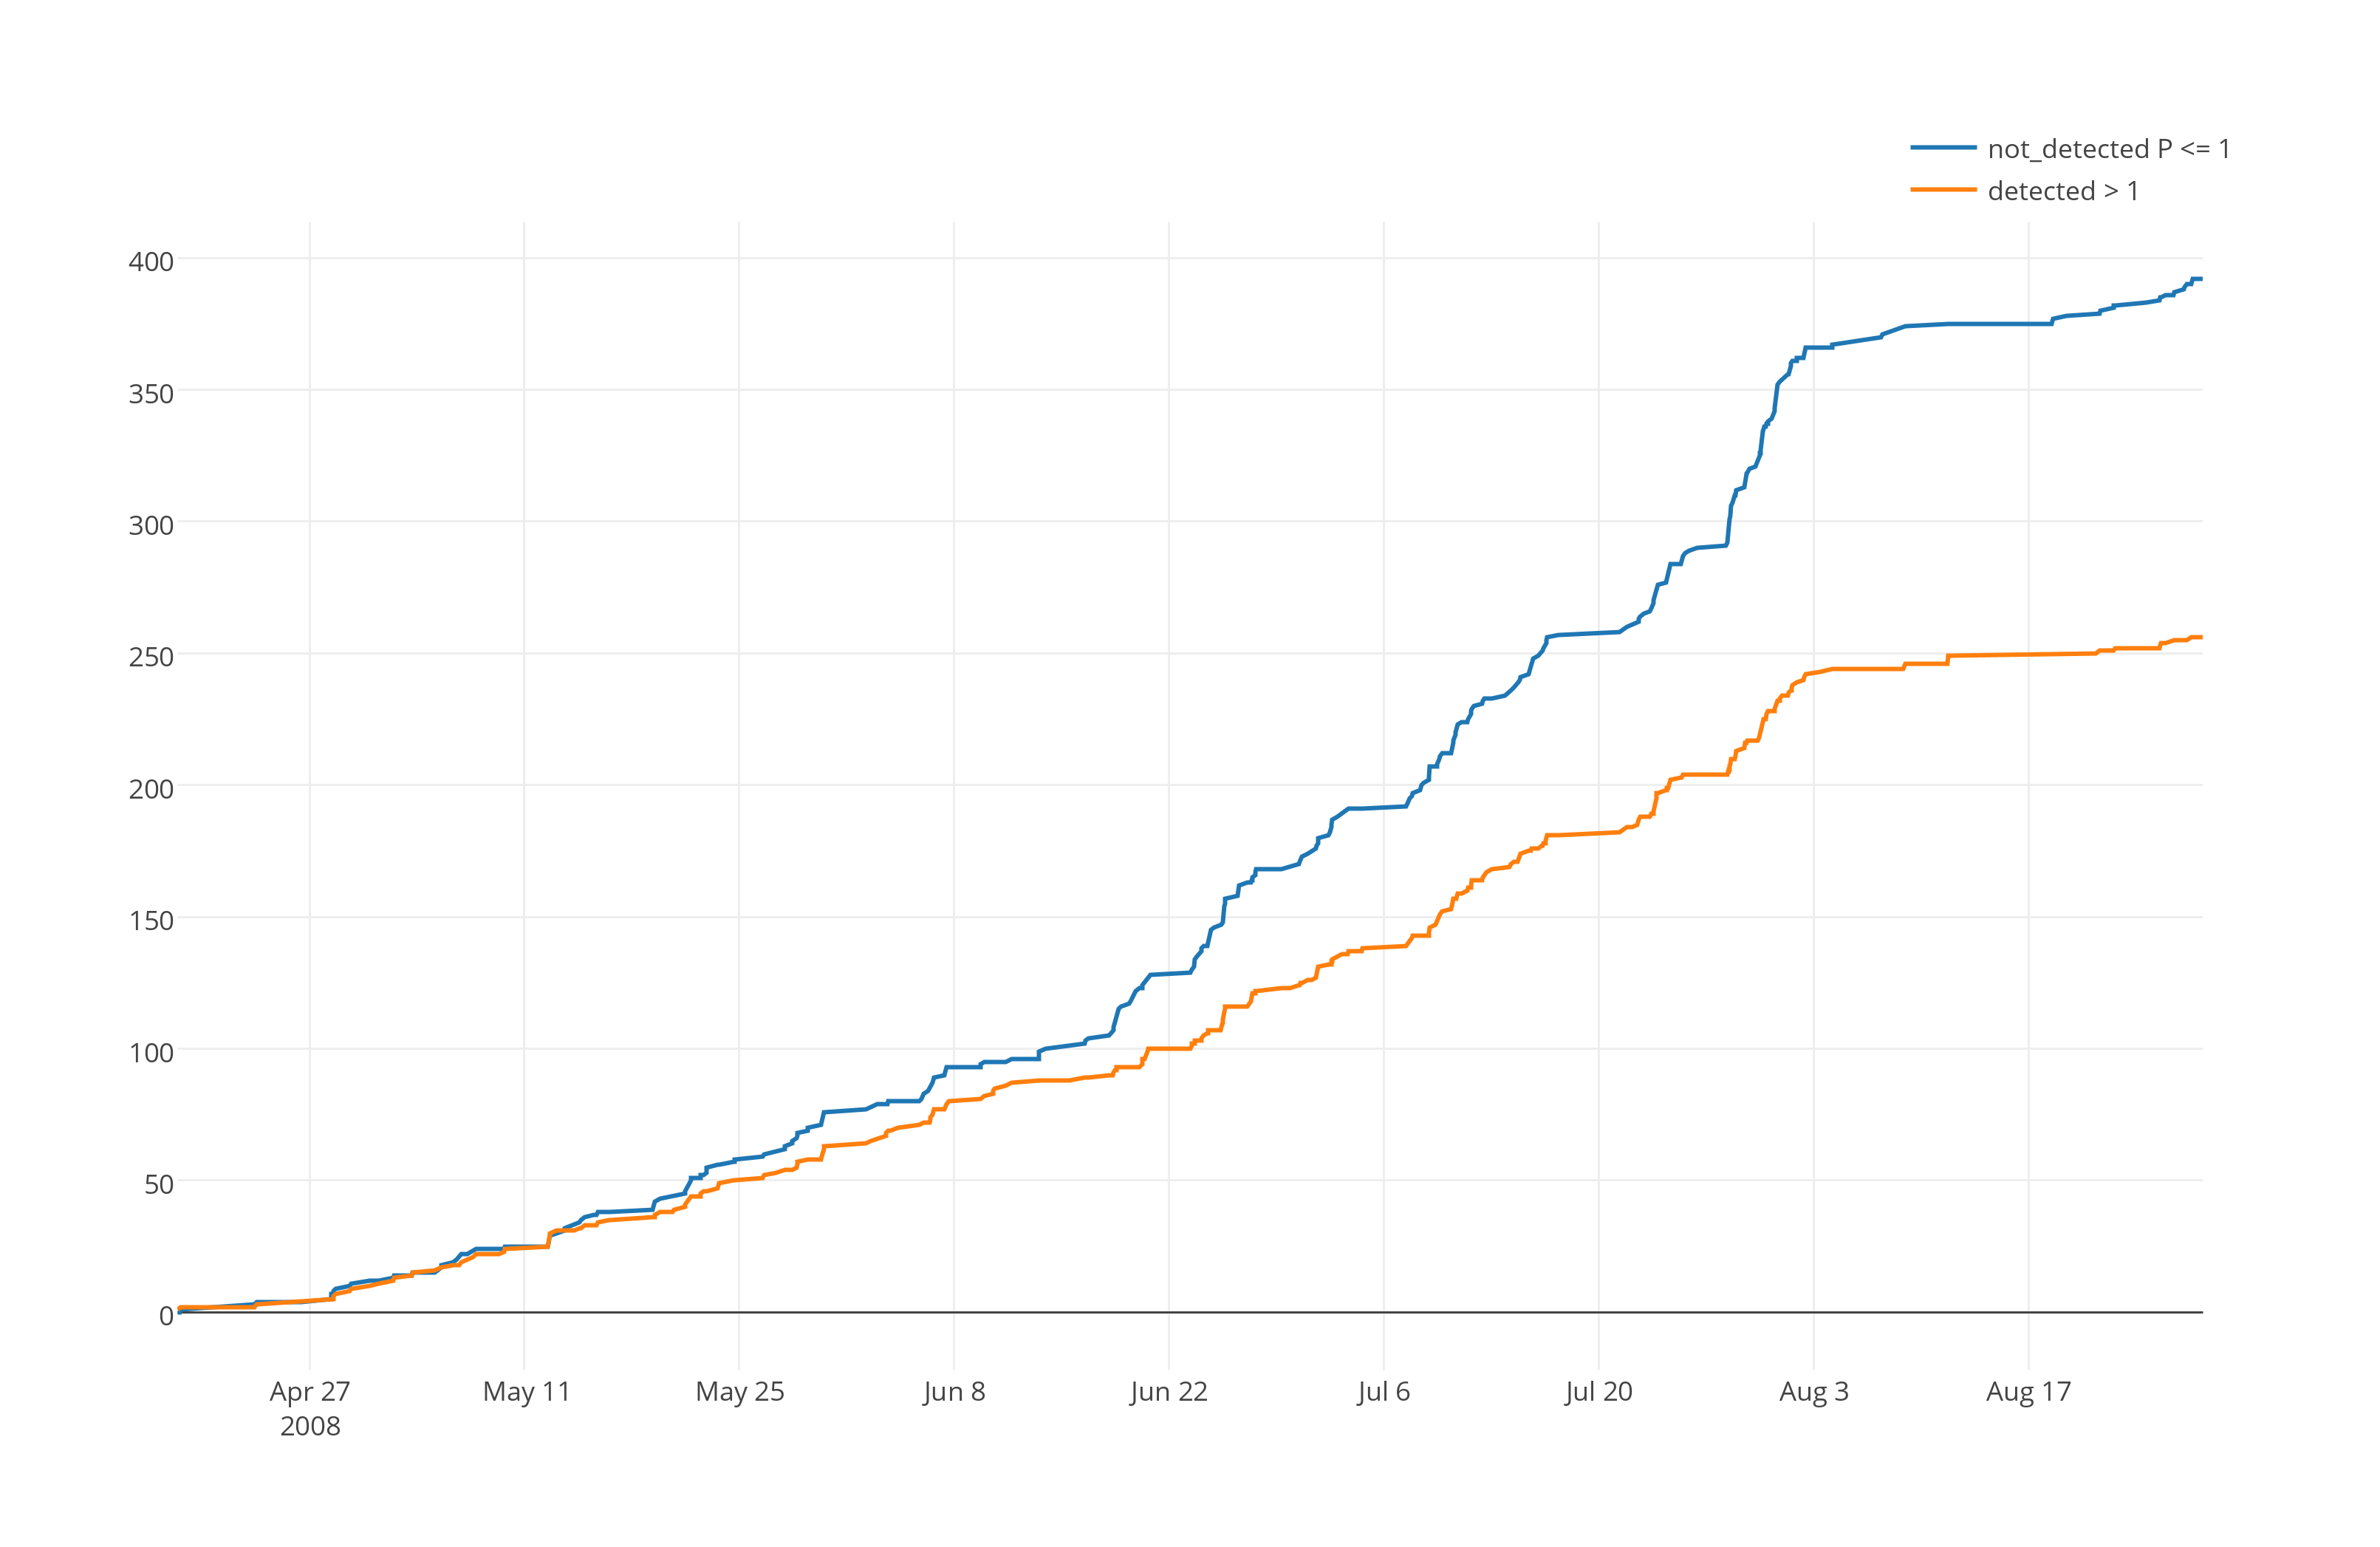
\includegraphics[scale=0.55]{media/bianca-13.png}
    \caption{{\tt BIANCA} warnings from April to August 2008 using the first normalization.
    \label{fig:bianca-exp-1}}
\end{figure}

With the first normalization, we {\tt BIANCA} raised 69,519 warnings out of 167,597 (41.5\%) commits we analyze. Out of these 69,519, 13.4\% turned out to be false positives. A false positive is a commit that have been tagged as introducing a bug by {\tt BIANCA} but did not according to the history. However, false positives have to deal with carefully in this study as the commit might have introduced a bug but the bug could have not been reported yet.

In our second experiment, we used the second normalization and {\tt BIANCA} raised 83,627 warnings out of 167,597 (48.89\%) commit we analyze. However, the false positive rate increases to 21\%. Figure \ref{fig:bianca-exp-2} shows the results.

\begin{figure}[h!]
  \centering
    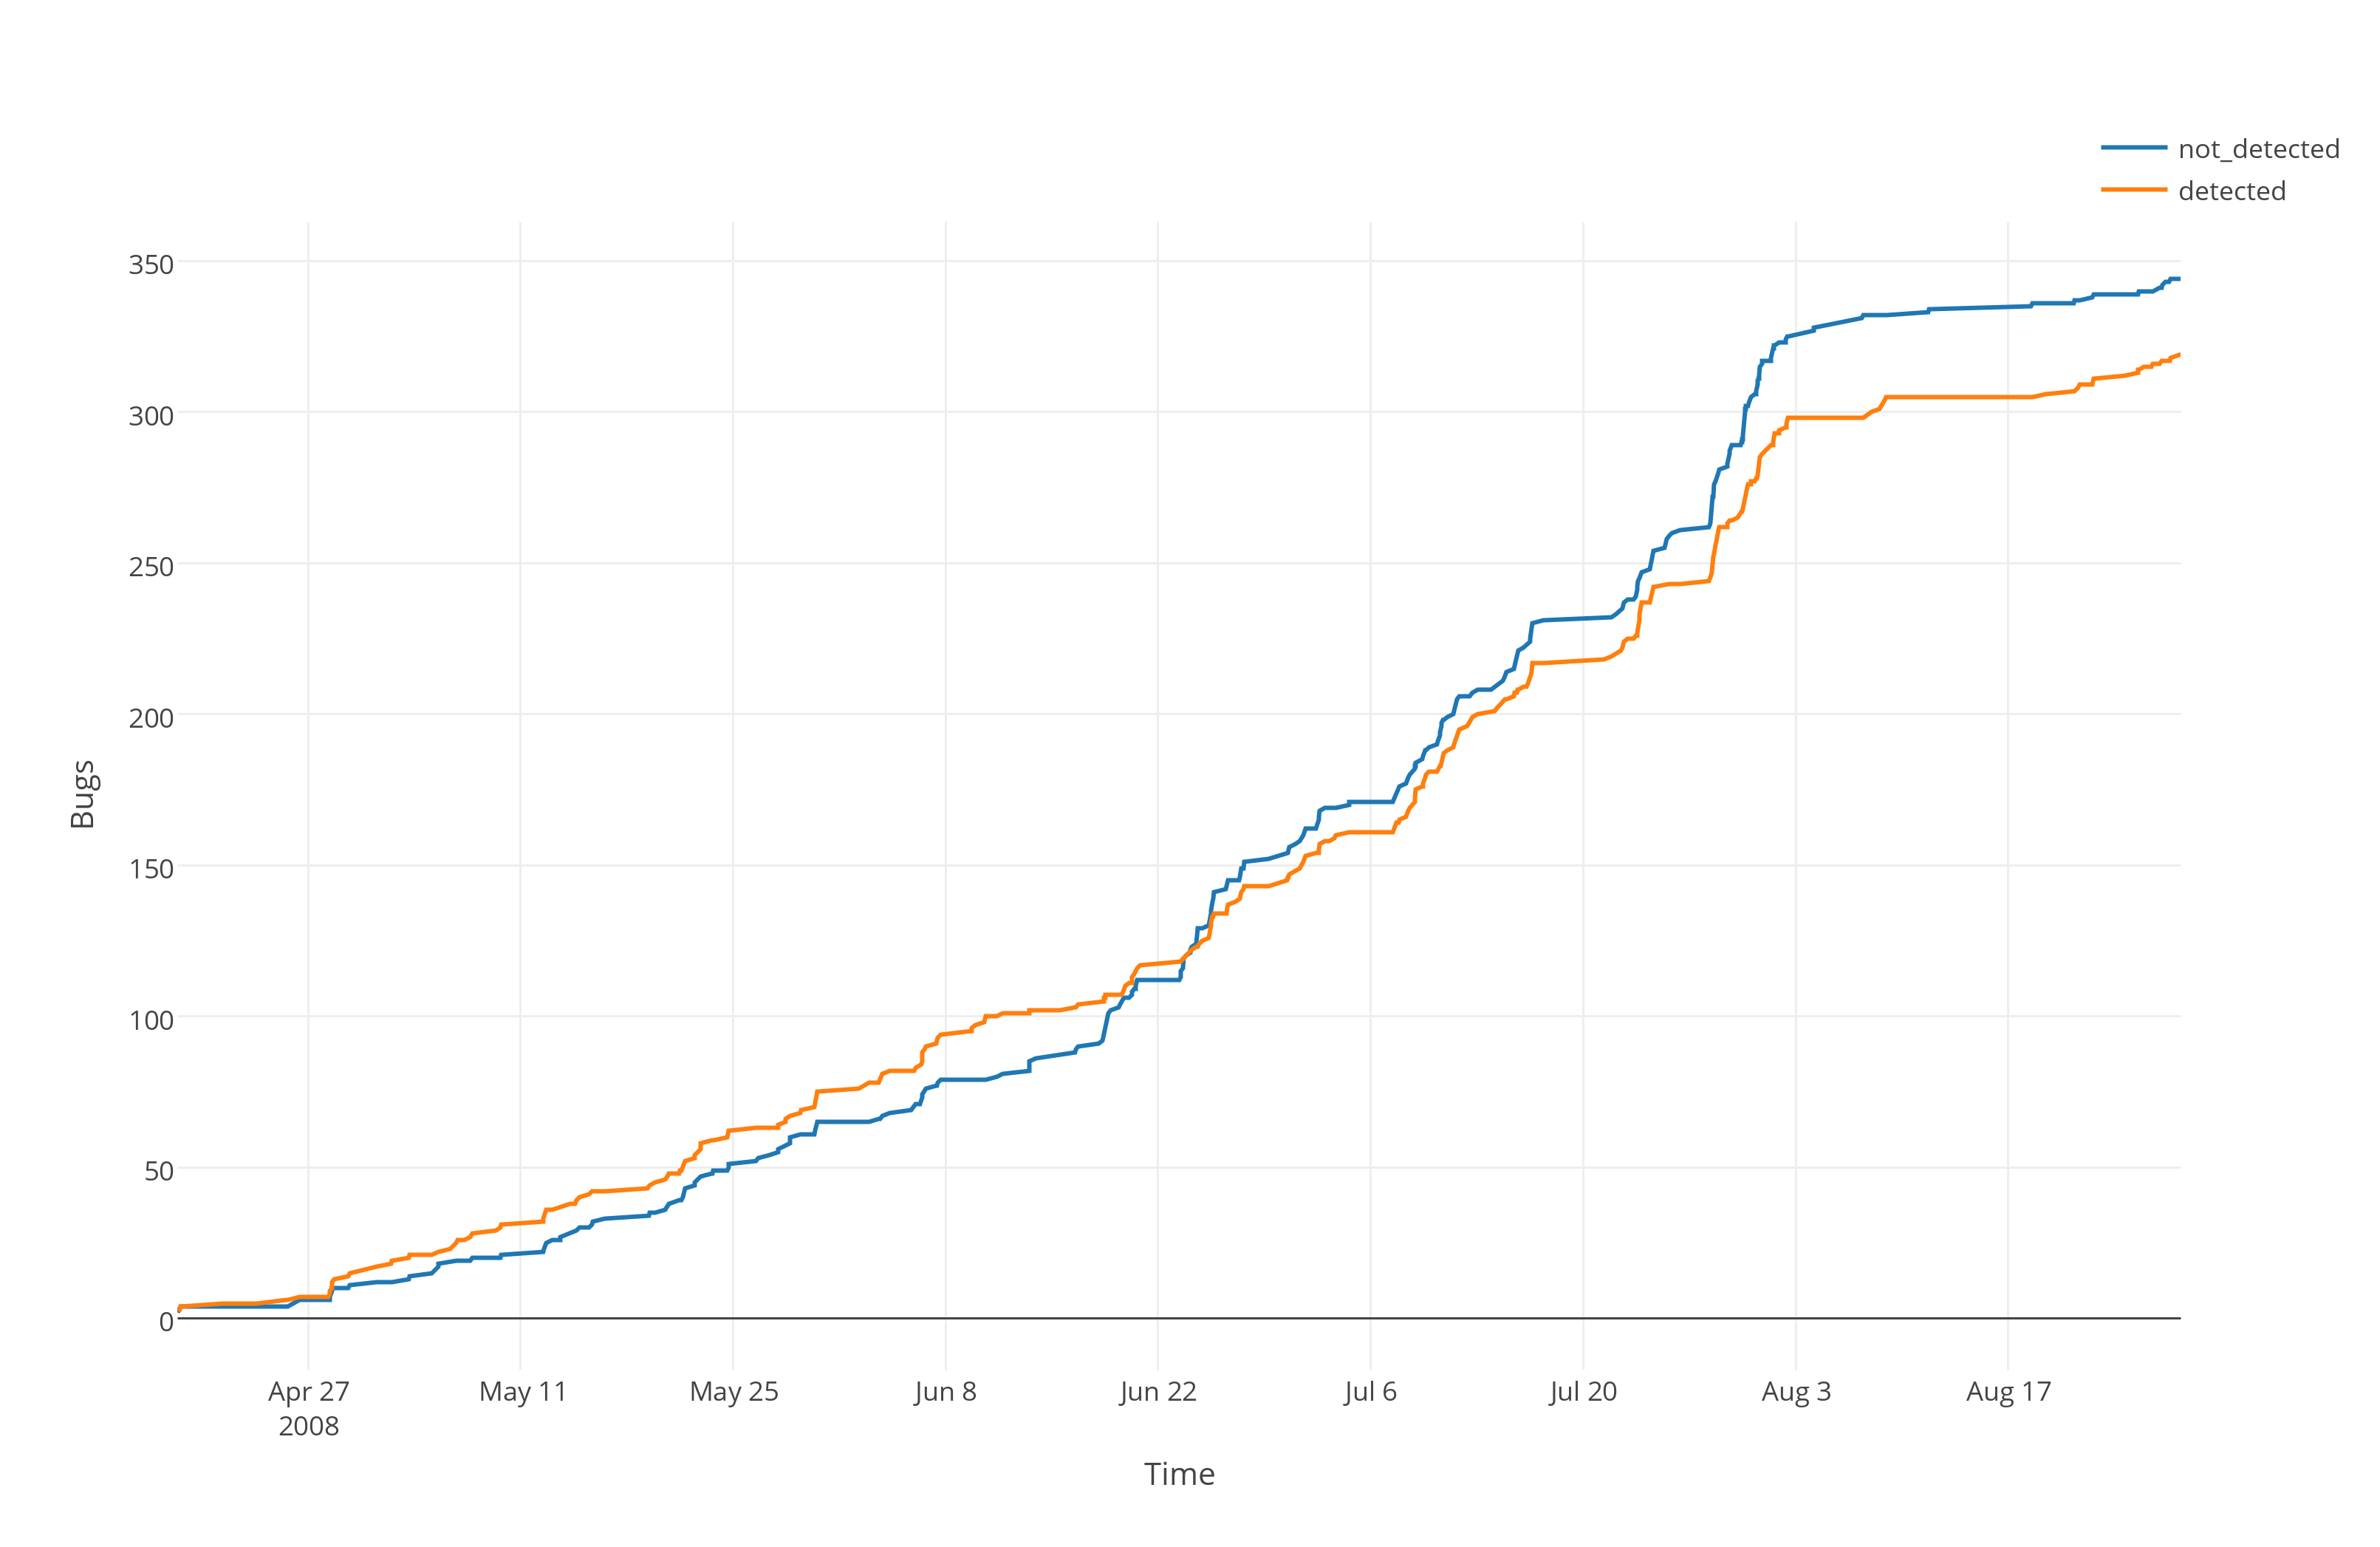
\includegraphics[scale=0.55]{media/bianca-20.png}
    \caption{{\tt BIANCA} warnings from April to August 2008 using the second normalization.
    \label{fig:bianca-exp-2}}
\end{figure}

\subsection{Planned experiments}

{\tt BIANCA} experiments are still in their early stage and we still trying to improve our normalizations in order to reduce the false positive rate. In addition to these improvements, we want to conduct the following additional experiments:

\begin{itemize}
	\item Full history test with Normalization 1.
	\item Full history test with Normalization 2.
	\item Full history test with Normalization 3.
	\item Full history test with Normalization 4.
	\item An human study where:
	\begin{itemize}
		\item  Developers use {\tt BIANCA} in order to determine whether or not developers take into account our warnings or override them.
		\item Rate the proposed solution in a scale from 1 to 10 in order to determine if the proposed change pattern does resolve the current problem.
	\end{itemize}
\end{itemize}
